A Inception-v3 modell sb-photothemes-imagenet114 adathalmazon teljes tanítással történt tesztelésének eredménye. Lásd a soron következő ábrákat és táblázatokat a mérések eredményeihez.

\subsubsection{Inception-v3 teljes tanítás folyamata}
\begin{itemize} 
	\item Epoch 1/10 - train: 2259/2259 [05:35<00:00,  6.72it/s]
	\item Epoch 1/10 - val: 282/282 [00:33<00:00,  8.52it/s]
	\item Epoch 1: Train loss=2.1448, acc=0.6042 Val loss=1.1183, acc=0.6850
	\item Epoch 2/10 - train: 2259/2259 [05:34<00:00,  6.74it/s]
	\item Epoch 2/10 - val: 282/282 [00:33<00:00,  8.52it/s]
	\item Epoch 2: Train loss=1.2943, acc=0.7373 Val loss=0.9889, acc=0.7210
	\item Epoch 3/10 - train: 2259/2259 [05:35<00:00,  6.74it/s]
	\item Epoch 3/10 - val: 282/282 [00:32<00:00,  8.55it/s]
	\item Epoch 3: Train loss=0.9102, acc=0.8097 Val loss=0.9692, acc=0.7399
	\item Epoch 4/10 - train: 2259/2259 [05:35<00:00,  6.74it/s]
	\item Epoch 4/10 - val: 282/282 [00:33<00:00,  8.53it/s]
	\item Epoch 4: Train loss=0.6552, acc=0.8592 Val loss=1.0133, acc=0.7404
	\item Epoch 5/10 - train: 2259/2259 [05:35<00:00,  6.73it/s]
	\item Epoch 5/10 - val: 282/282 [00:32<00:00,  8.57it/s]
	\item Epoch 5: Train loss=0.4818, acc=0.8953 Val loss=1.0527, acc=0.7486
	\item Epoch 6/10 - train: 2259/2259 [05:35<00:00,  6.73it/s]
	\item Epoch 6/10 - val: 282/282 [00:33<00:00,  8.49it/s]
	\item Epoch 6: Train loss=0.3864, acc=0.9153 Val loss=1.1098, acc=0.7539
	\item Epoch 7/10 - train: 2259/2259 [05:35<00:00,  6.74it/s]
	\item Epoch 7/10 - val: 282/282 [00:32<00:00,  8.58it/s]
	\item Epoch 7: Train loss=0.3178, acc=0.9298 Val loss=1.1535, acc=0.7513
	\item Epoch 8/10 - train: 2259/2259 [05:35<00:00,  6.74it/s]
	\item Epoch 8/10 - val: 282/282 [00:33<00:00,  8.47it/s]
	\item Epoch 8: Train loss=0.2772, acc=0.9386 Val loss=1.1772, acc=0.7514
	\item Epoch 9/10 - train: 2259/2259 [05:35<00:00,  6.74it/s]
	\item Epoch 9/10 - val: 282/282 [00:32<00:00,  8.57it/s]
	\item Epoch 9: Train loss=0.2435, acc=0.9464 Val loss=1.2565, acc=0.7496
	\item Epoch 10/10 - train: 2259/2259 [05:35<00:00,  6.73it/s]
	\item Epoch 10/10 - val: 282/282 [00:33<00:00,  8.50it/s]
	\item Epoch 10: Train loss=0.2234, acc=0.9502 Val loss=1.2737, acc=0.7524
\end{itemize}

\subsubsection{Inception-v3 teljes tanítás folyamata}
  \begin{figure}[H]
    \centering
    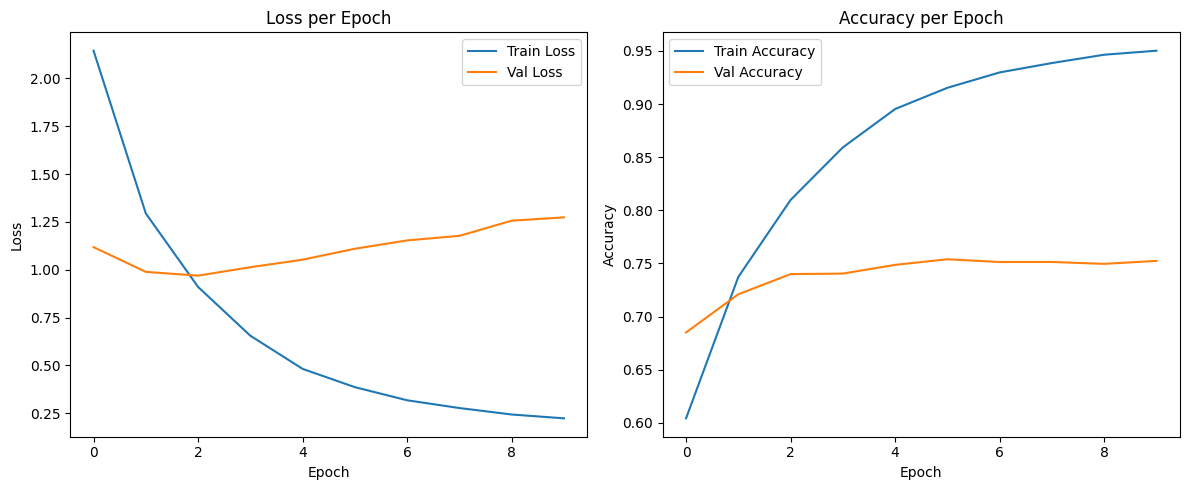
\includegraphics[width=1.0\textwidth]{images/phase02/Inception-v3_learning_curve.png}
    \caption{Inception-v3 teljes tanítás utáni sima Confusion Mátrix}
    \label{fig:phase02_Inception-v3_learning_curves}
  \end{figure}

\subsubsection{Inception-v3 teljes tanítás utáni eredményei}
  \begin{center}
  \begin{longtable}{l c}
  \caption{Inception-v3 teljes tanítás utáni vizsgálati eredményei} \label{tab:phase02_Inception-v3} \\
  \toprule
  \textbf{Metrika} & \textbf{Érték} \\
  \midrule
  \endfirsthead
  \toprule
  \textbf{Metrika} & \textbf{Érték} \\
  \midrule
  \endhead
  Top-1 Accuracy & 0.7518 \\
  Top-5 Accuracy & 0.9320 \\
  Precision & 0.6963 \\
  Recall & 0.6787 \\
  F1-score & 0.6908 \\
  Inference time & 25.11 sec \\
  \bottomrule
  \end{longtable}
  \end{center}

\subsubsection{Inception-v3 eredményeinek összehasonlítása}
  \begin{center}
  \begin{longtable}{l c c}
  \caption{Inception-v3 eredményeinek összehasonlítása} \label{tab:phase02_Inception-v3_compare} \\
  \toprule
  \textbf{Metrika} & \textbf{Pretrained} & \textbf{Fine-tuned} \\
  \midrule
  \endfirsthead
  \toprule
  \textbf{Metrika} & \textbf{Pretrained} & \textbf{Fine-tuned} \\
  \midrule
  \endhead
  Top-1 Accuracy  & 0.4763 & 0.7518 \\
  Top-5 Accuracy & 0.8008 & 0.9320 \\
  Precision & 0.3833 & 0.6963 \\
  Recall & 0.3896 & 0.6787 \\
  F1-score & 0.3683 & 0.6827 \\
  Inference time & 38.06 sec & 33.62 sec \\
  \bottomrule
  \end{longtable}
  \end{center}

\subsubsection{Inception-v3 eredményeinek összehasonlítása}
  \begin{figure}[H]
    \centering
    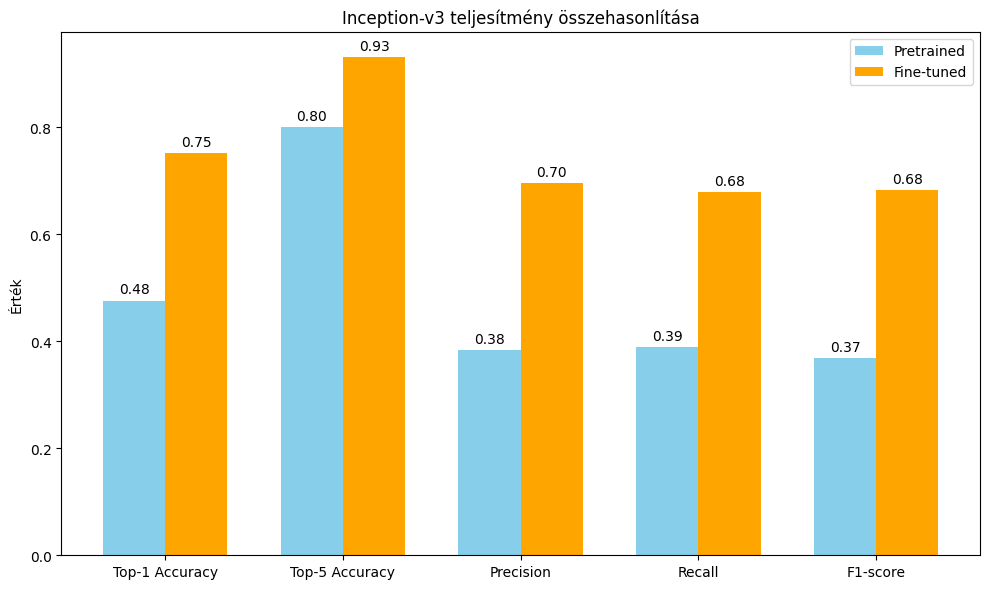
\includegraphics[width=1.0\textwidth]{images/phase02/Inception-v3_compare01.png}
    \caption{Inception-v3 eredményeinek összehasonlítása}
    \label{fig:Inception-v3_compare01}
  \end{figure}

\subsubsection{Inception-v3 eredményeinek összehasonlítása}
  \begin{figure}[H]
    \centering
    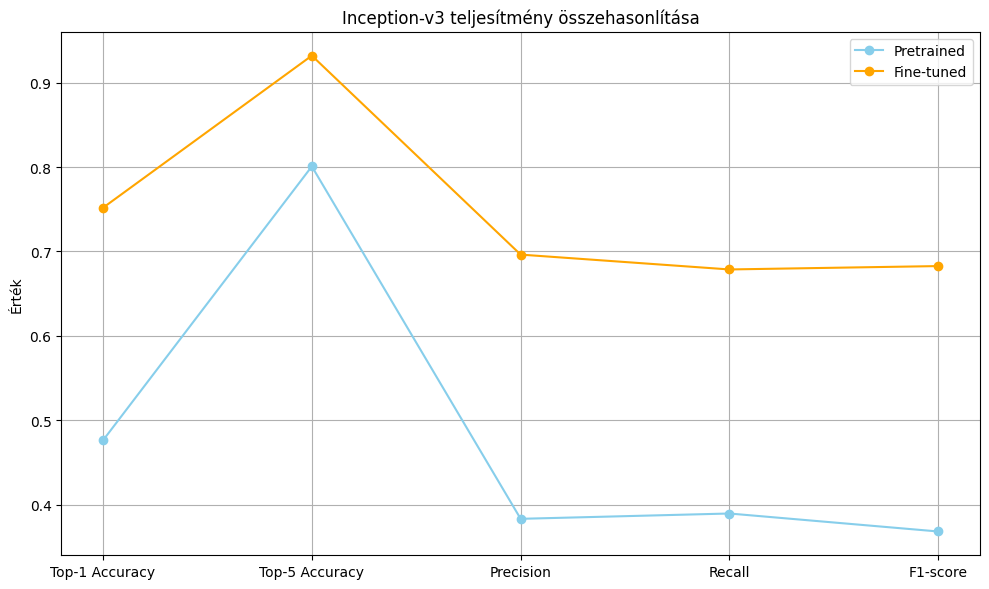
\includegraphics[width=1.0\textwidth]{images/phase02/Inception-v3_compare02.png}
    \caption{Inception-v3 eredményeinek összehasonlítása}
    \label{fig:Inception-v3_compare02}
  \end{figure}

\subsubsection{Inception-v3 teljes tanítás utáni sima Confusion Mátrix}
  \begin{figure}[H]
    \centering
    
\includegraphics[width=1.0\textwidth]{images/phase02/Inception-v3_basic_conf_mat.png}
    \caption{Inception-v3 teljes tanítás utáni sima Confusion Mátrix}
    \label{fig:phase02_Inception-v3_basic_conf_mat}
  \end{figure}

  \subsubsection{Inception-v3 Confusion Mátrixok összehasonlítása}
  \begin{figure}[H]
    \centering
    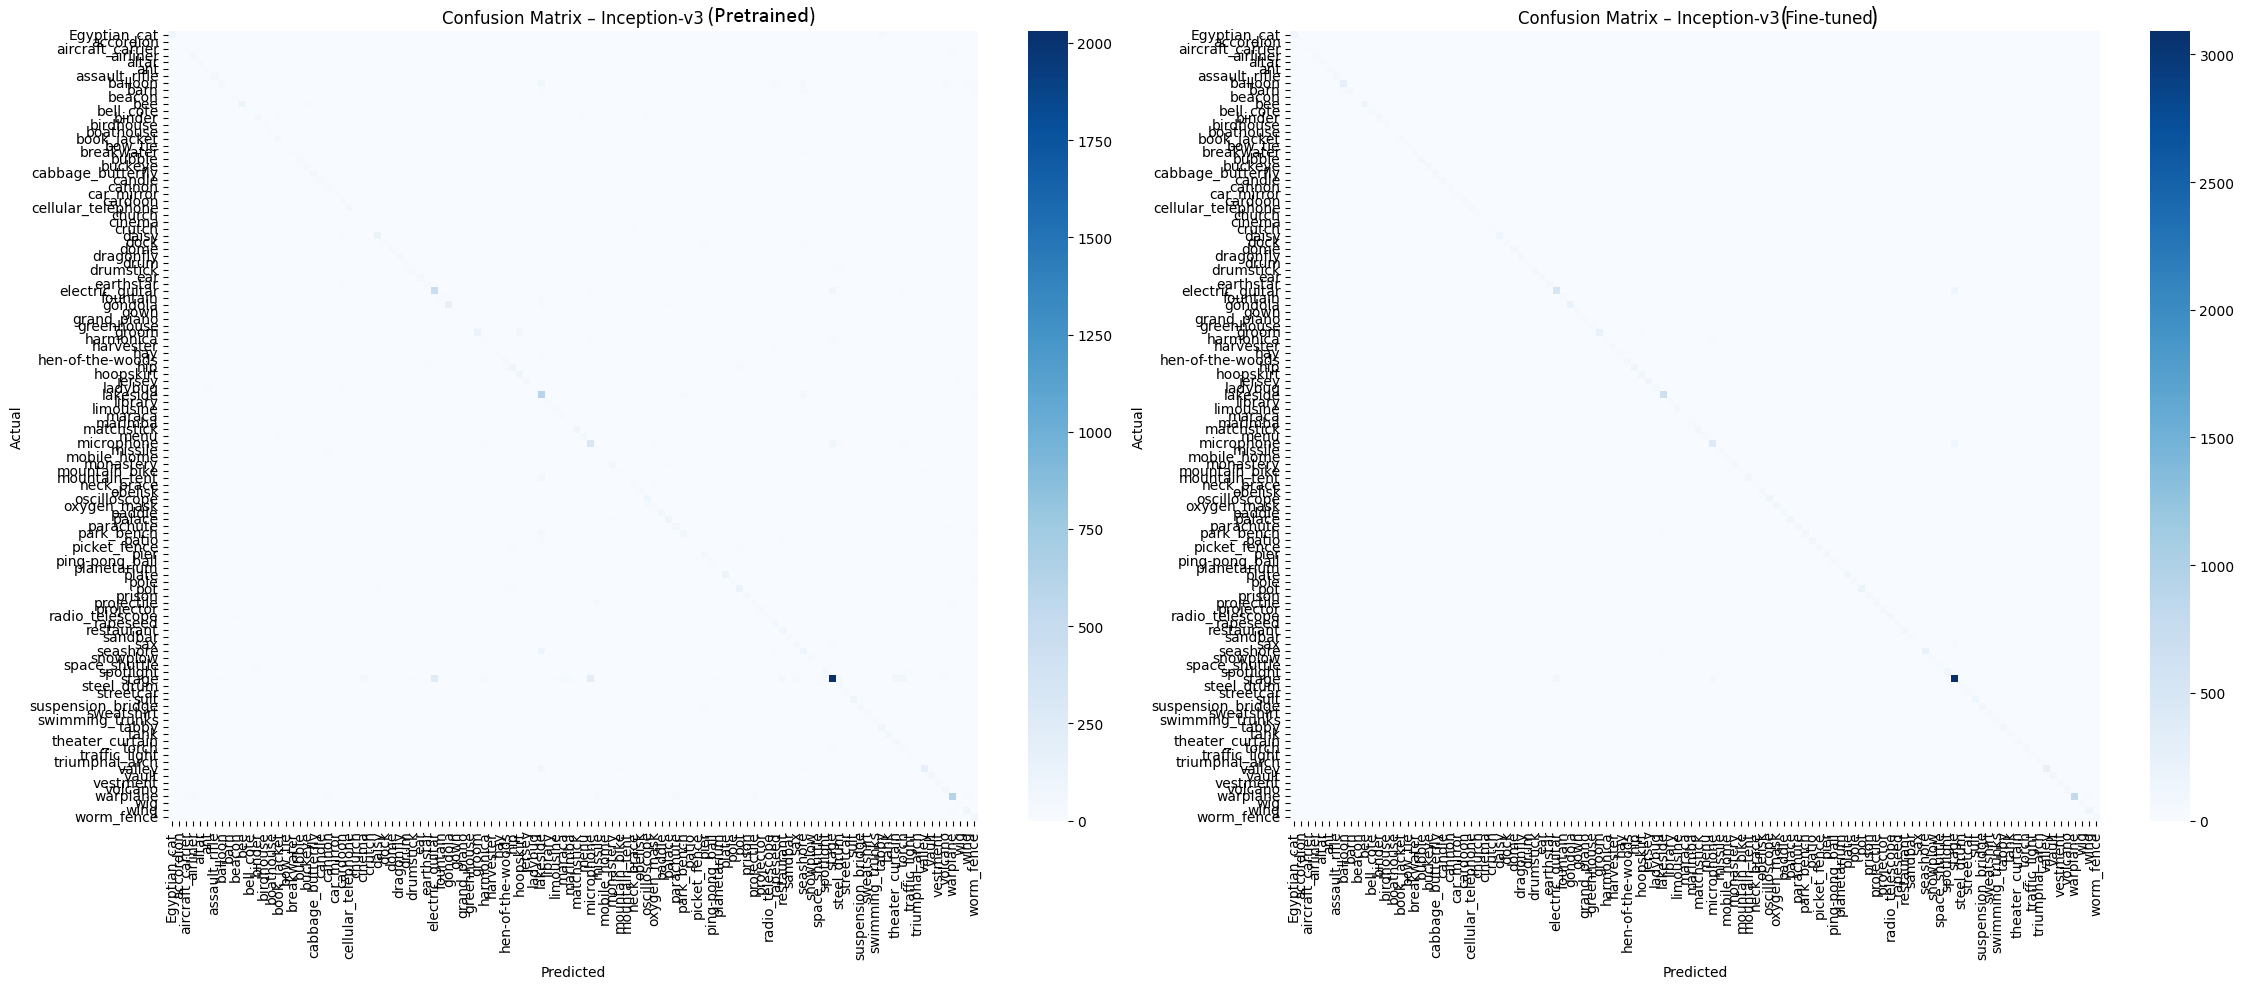
\includegraphics[width=1.0\textwidth]{images/phase02/Inception-v3_basic_conf_mat_compare.png}
    \caption{Inception-v3 sima Confusion Mátrixok összehasonlítása}
    \label{fig:phase02_Inception-v3_basic_conf_mat_compare}
  \end{figure}

  \subsubsection{Inception-v3 teljes tanítás utáni normalizált Confusion Mátrix}
  \begin{figure}[H]
    \centering
    
\includegraphics[width=1.0\textwidth]{images/phase02/Inception-v3_normalised_conf_mat.png}
    \caption{Inception-v3 teljes tanítás utáni normalizált Confusion Mátrix}
    \label{fig:phase02_Inception-v3_normalised_conf_mat}
  \end{figure}

  \subsubsection{Inception-v3 normalizált Confusion Mátrixok összehasonlítása}
  \begin{figure}[H]
    \centering
    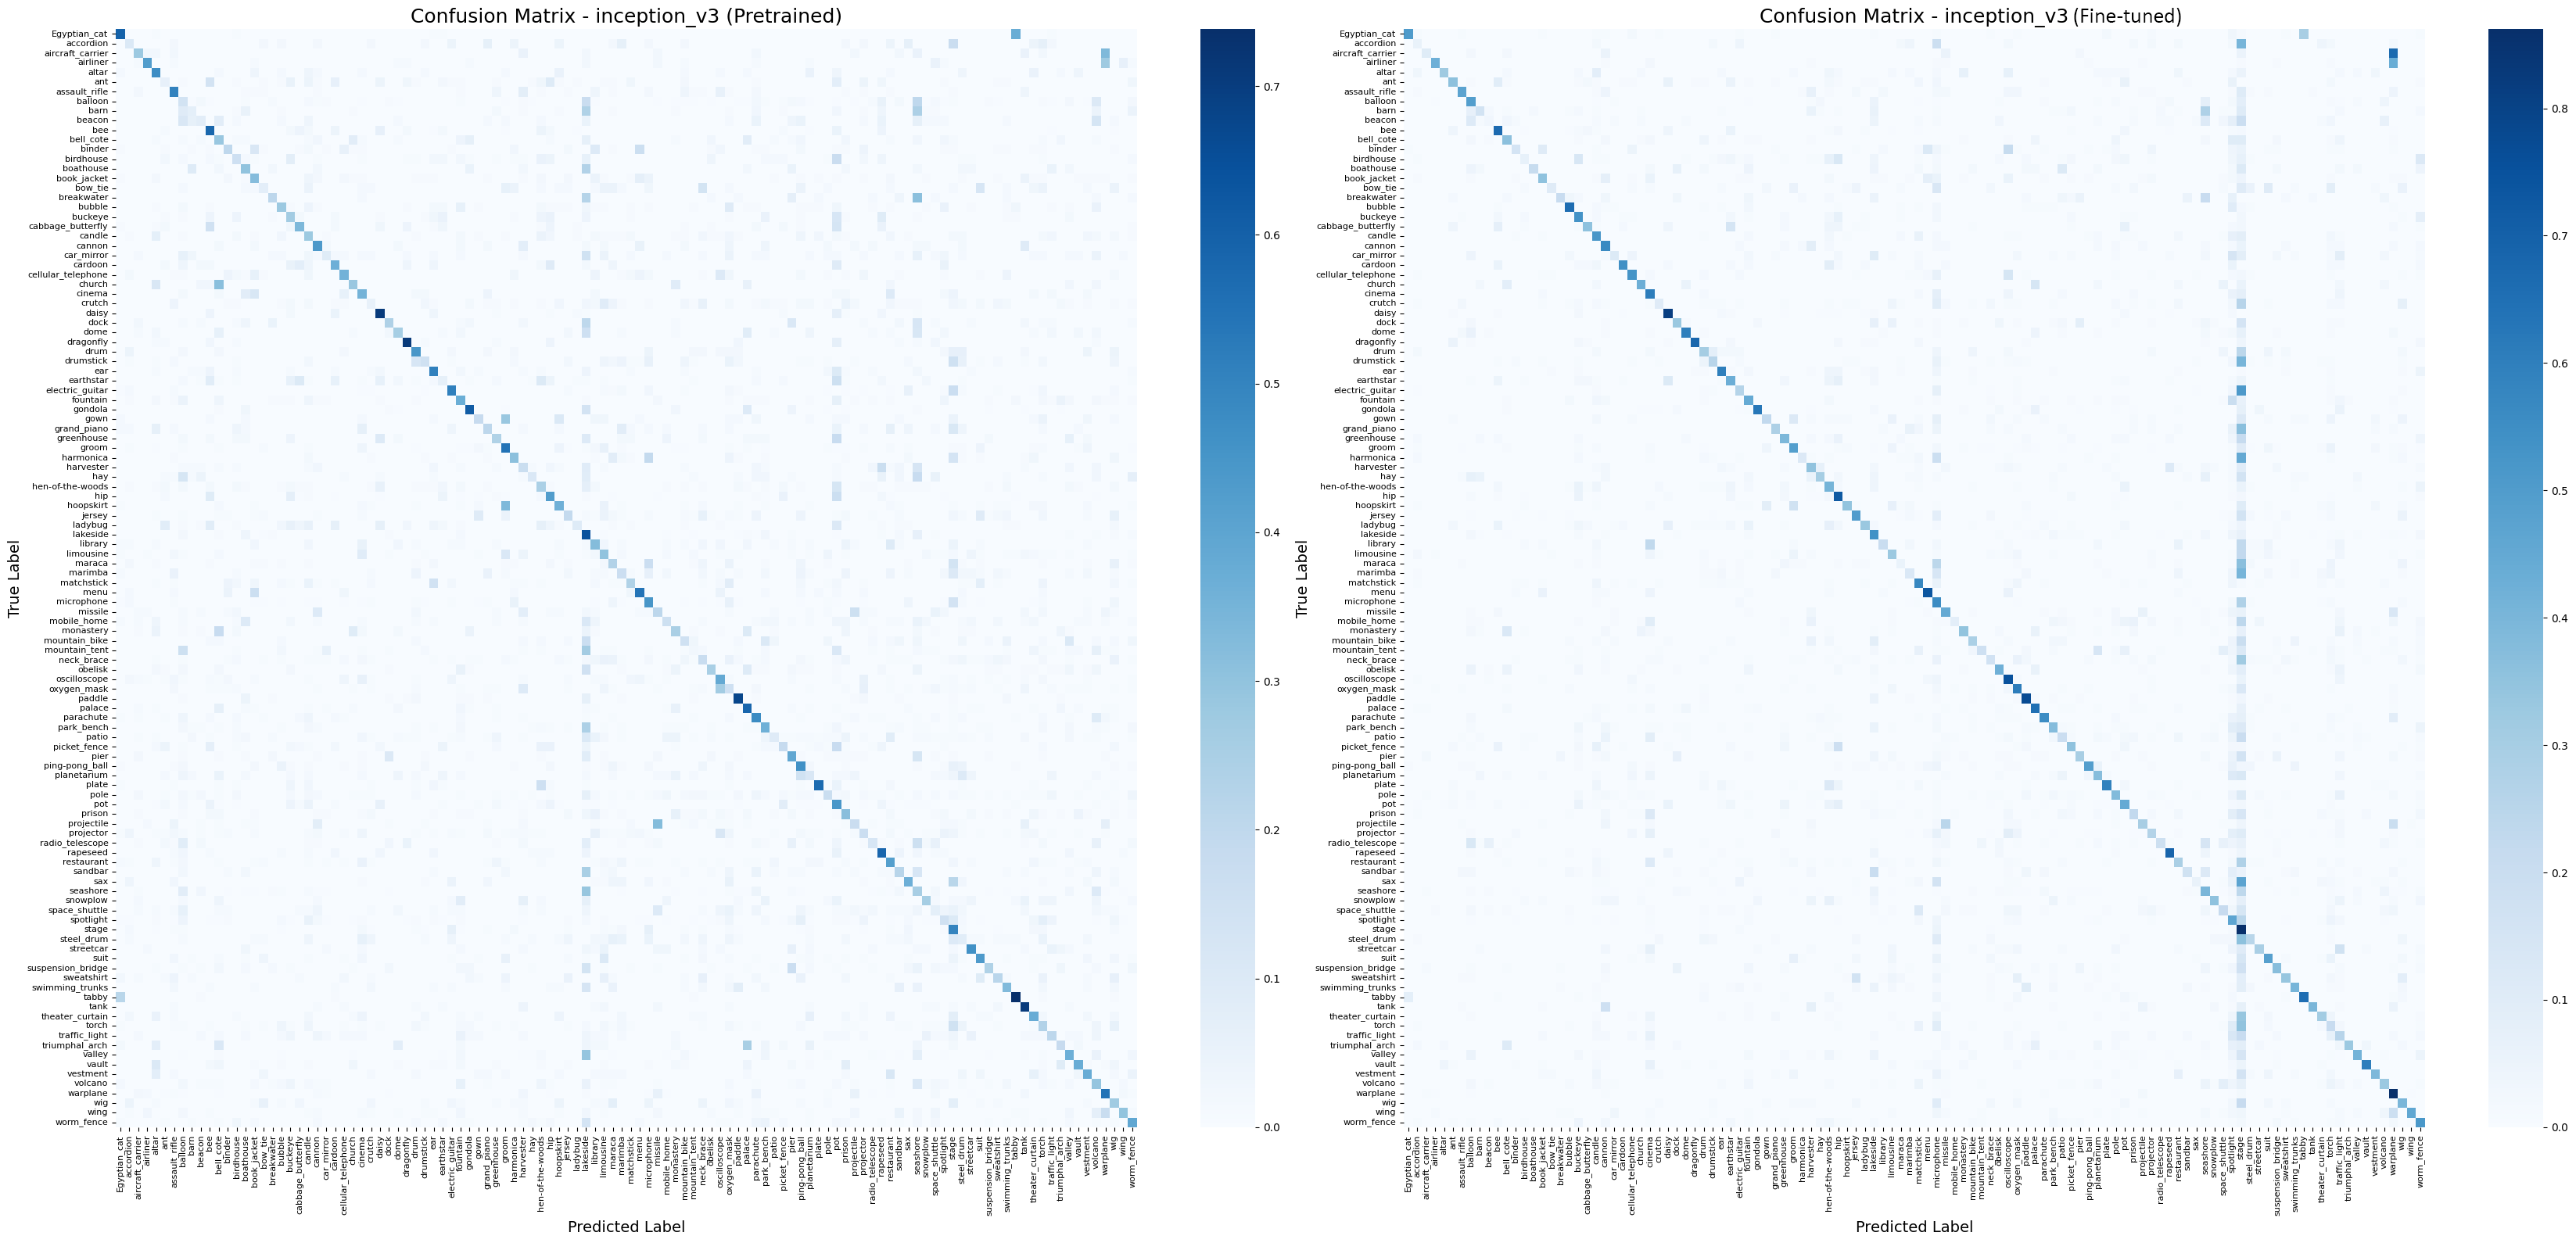
\includegraphics[width=1.0\textwidth]{images/phase02/Inception-v3_normalised_conf_mat_compare.png}
    \caption{Inception-v3 normalizált Confusion Mátrixok összehasonlítása}
    \label{fig:phase02_Inception-v3_normalised_conf_mat_compare}
  \end{figure}

\subsubsection{Inception-v3 teljes tanítás utáni részletes osztályonkénti metrikák}
  \begin{center}
\begin{longtable}{lllll}
\caption{Inception-v3 teljes tanítás utáni részletes osztályonkénti metrikák}\label{tab:phase2_Inception-v3_class_table}\\
\toprule
class & precision & recall & f1-score & support \\
\midrule
\endfirsthead
\toprule
class & precision & recall & f1-score & support \\
\midrule
\endhead
gondola & 0.95 & 0.92 & 0.93 & 227 \\
airliner & 0.91 & 0.64 & 0.75 & 80 \\
warplane & 0.91 & 0.92 & 0.92 & 871 \\
plate & 0.90 & 0.91 & 0.91 & 143 \\
assault-rifle & 0.89 & 0.78 & 0.83 & 91 \\
valley & 0.89 & 0.79 & 0.84 & 295 \\
vault & 0.89 & 0.83 & 0.86 & 104 \\
Egyptian-cat & 0.87 & 0.79 & 0.83 & 145 \\
tank & 0.87 & 0.77 & 0.82 & 78 \\
dragonfly & 0.86 & 0.83 & 0.84 & 75 \\
paddle & 0.85 & 0.90 & 0.88 & 93 \\
drumstick & 0.84 & 0.64 & 0.73 & 126 \\
ear & 0.84 & 0.81 & 0.83 & 80 \\
groom & 0.84 & 0.76 & 0.80 & 285 \\
palace & 0.84 & 0.81 & 0.82 & 139 \\
stage & 0.84 & 0.91 & 0.87 & 3380 \\
breakwater & 0.83 & 0.67 & 0.74 & 58 \\
pot & 0.83 & 0.67 & 0.74 & 254 \\
wing & 0.83 & 0.80 & 0.82 & 148 \\
lakeside & 0.82 & 0.84 & 0.83 & 801 \\
altar & 0.80 & 0.68 & 0.73 & 59 \\
greenhouse & 0.80 & 0.69 & 0.74 & 51 \\
picket-fence & 0.80 & 0.59 & 0.68 & 118 \\
rapeseed & 0.80 & 0.77 & 0.78 & 77 \\
tabby & 0.80 & 0.83 & 0.82 & 107 \\
bee & 0.79 & 0.78 & 0.78 & 212 \\
oscilloscope & 0.79 & 0.82 & 0.80 & 143 \\
ping-pong-ball & 0.79 & 0.64 & 0.71 & 91 \\
swimming-trunks & 0.79 & 0.72 & 0.75 & 79 \\
daisy & 0.78 & 0.90 & 0.84 & 149 \\
mountain-tent & 0.78 & 0.81 & 0.80 & 121 \\
projectile & 0.78 & 0.72 & 0.75 & 117 \\
electric-guitar & 0.77 & 0.74 & 0.76 & 687 \\
suspension-bridge & 0.77 & 0.74 & 0.76 & 127 \\
bubble & 0.76 & 0.78 & 0.77 & 100 \\
parachute & 0.76 & 0.80 & 0.78 & 117 \\
seashore & 0.76 & 0.79 & 0.77 & 289 \\
suit & 0.76 & 0.82 & 0.79 & 141 \\
hip & 0.75 & 0.77 & 0.76 & 195 \\
matchstick & 0.75 & 0.77 & 0.76 & 127 \\
menu & 0.75 & 0.84 & 0.79 & 68 \\
restaurant & 0.75 & 0.76 & 0.75 & 141 \\
balloon & 0.74 & 0.77 & 0.76 & 338 \\
bow-tie & 0.74 & 0.48 & 0.58 & 67 \\
church & 0.74 & 0.71 & 0.72 & 35 \\
microphone & 0.74 & 0.68 & 0.71 & 596 \\
monastery & 0.74 & 0.71 & 0.72 & 112 \\
triumphal-arch & 0.74 & 0.73 & 0.73 & 55 \\
barn & 0.73 & 0.66 & 0.69 & 111 \\
hoopskirt & 0.73 & 0.84 & 0.78 & 135 \\
mobile-home & 0.73 & 0.52 & 0.61 & 83 \\
oxygen-mask & 0.73 & 0.78 & 0.75 & 143 \\
park-bench & 0.73 & 0.66 & 0.69 & 144 \\
theater-curtain & 0.73 & 0.64 & 0.68 & 80 \\
cardoon & 0.72 & 0.76 & 0.74 & 55 \\
dock & 0.72 & 0.68 & 0.70 & 84 \\
dome & 0.72 & 0.85 & 0.78 & 85 \\
birdhouse & 0.71 & 0.45 & 0.55 & 116 \\
jersey & 0.71 & 0.77 & 0.74 & 154 \\
snowplow & 0.71 & 0.73 & 0.72 & 62 \\
limousine & 0.70 & 0.65 & 0.67 & 119 \\
bell-cote & 0.69 & 0.66 & 0.68 & 77 \\
cabbage-butterfly & 0.69 & 0.69 & 0.69 & 101 \\
gown & 0.69 & 0.56 & 0.62 & 66 \\
library & 0.69 & 0.55 & 0.62 & 74 \\
radio-telescope & 0.69 & 0.73 & 0.71 & 108 \\
steel-drum & 0.69 & 0.56 & 0.62 & 84 \\
candle & 0.68 & 0.71 & 0.69 & 111 \\
cellular-telephone & 0.68 & 0.73 & 0.71 & 104 \\
streetcar & 0.67 & 0.72 & 0.70 & 65 \\
mountain-bike & 0.66 & 0.50 & 0.57 & 66 \\
pier & 0.66 & 0.66 & 0.66 & 97 \\
wig & 0.66 & 0.54 & 0.59 & 70 \\
worm-fence & 0.66 & 0.73 & 0.69 & 137 \\
spotlight & 0.65 & 0.54 & 0.59 & 202 \\
drum & 0.64 & 0.71 & 0.67 & 49 \\
book-jacket & 0.63 & 0.60 & 0.61 & 90 \\
fountain & 0.63 & 0.60 & 0.61 & 92 \\
ladybug & 0.63 & 0.66 & 0.65 & 108 \\
prison & 0.63 & 0.62 & 0.63 & 101 \\
projector & 0.63 & 0.52 & 0.57 & 157 \\
sweatshirt & 0.63 & 0.69 & 0.66 & 80 \\
neck-brace & 0.62 & 0.44 & 0.51 & 137 \\
obelisk & 0.62 & 0.68 & 0.65 & 95 \\
planetarium & 0.62 & 0.56 & 0.59 & 62 \\
harmonica & 0.61 & 0.33 & 0.43 & 100 \\
volcano & 0.61 & 0.66 & 0.63 & 119 \\
aircraft-carrier & 0.60 & 0.62 & 0.61 & 39 \\
hay & 0.59 & 0.67 & 0.63 & 73 \\
patio & 0.59 & 0.59 & 0.59 & 144 \\
vestment & 0.59 & 0.84 & 0.69 & 69 \\
beacon & 0.58 & 0.50 & 0.54 & 62 \\
car-mirror & 0.58 & 0.56 & 0.57 & 68 \\
crutch & 0.58 & 0.47 & 0.52 & 105 \\
binder & 0.57 & 0.70 & 0.63 & 105 \\
buckeye & 0.57 & 0.69 & 0.63 & 101 \\
grand-piano & 0.57 & 0.60 & 0.58 & 63 \\
harvester & 0.57 & 0.63 & 0.60 & 71 \\
missile & 0.57 & 0.71 & 0.63 & 82 \\
pole & 0.55 & 0.58 & 0.56 & 136 \\
sandbar & 0.55 & 0.67 & 0.61 & 83 \\
space-shuttle & 0.55 & 0.55 & 0.55 & 84 \\
ant & 0.53 & 0.55 & 0.54 & 95 \\
hen-of-the-woods & 0.52 & 0.65 & 0.58 & 105 \\
sax & 0.50 & 0.32 & 0.39 & 112 \\
maraca & 0.49 & 0.27 & 0.35 & 90 \\
torch & 0.49 & 0.53 & 0.51 & 116 \\
cannon & 0.48 & 0.78 & 0.60 & 55 \\
earthstar & 0.48 & 0.69 & 0.57 & 121 \\
marimba & 0.47 & 0.48 & 0.48 & 79 \\
boathouse & 0.46 & 0.58 & 0.52 & 43 \\
cinema & 0.44 & 0.63 & 0.52 & 51 \\
accordion & 0.38 & 0.28 & 0.32 & 47 \\
traffic-light & 0.32 & 0.43 & 0.37 & 58 \\
\midrule
accuracy &  &  & 0.75 & 18172 \\
macro-avg & 0.70 & 0.68 & 0.68 & 18172 \\
weighted-avg & 0.75 & 0.75 & 0.75 & 18172 \\
\bottomrule
\end{longtable}
\end{center}


\subsubsection{GPU memóriahasználat}
\begin{itemize}
  \item aktív GPU: NVIDIA A100-SXM4-40GB
  \item GPU memória (lefoglalt): 1.3 GB
  \item GPU memória (használt):  0.32 GB
\end{itemize}

\subsubsection{Legrosszabbul teljesítő osztályok}
  \begin{center}
    \begin{longtable}{llll}
    \caption{Legrosszabbul teljesítő osztályok}\label{tab:phase02_Inception-v3_legrosszabb_osztlyok}\\
    \toprule
    Class & Precision & Recall & F1-score \\
    \midrule
    \endfirsthead
    \toprule
    Class & Precision & Recall & F1-score \\
    \midrule
    \endhead
    traffic-light & 0.32 & 0.43 & 0.37 \\
    accordion & 0.38 & 0.28 & 0.32 \\
    boathouse & 0.46 & 0.58 & 0.52 \\
    marimba & 0.47 & 0.48 & 0.48 \\
    maraca & 0.49 & 0.27 & 0.35 \\
    torch & 0.49 & 0.53 & 0.51 \\
    sax & 0.50 & 0.32 & 0.39 \\
    crutch & 0.58 & 0.47 & 0.52 \\
    harmonica & 0.61 & 0.33 & 0.43 \\
    neck-brace & 0.62 & 0.44 & 0.51 \\
    \bottomrule
    \end{longtable}
  \end{center}
  